\documentclass[letterpaper]{article}
\usepackage[submission]{aaai2026}
\usepackage{times}
\usepackage{helvet}
\usepackage{courier}
\usepackage[hyphens]{url}
\usepackage{graphicx}
\usepackage{natbib}
\urlstyle{rm}
\def\UrlFont{\rm}
\usepackage{caption}
\frenchspacing
\setlength{\pdfpagewidth}{8.5in}
\setlength{\pdfpageheight}{11in}
\usepackage{amsmath}
\usepackage{amssymb}
\usepackage{booktabs}
\usepackage{multirow}
\usepackage{tikz}
\usepackage{placeins}
\usetikzlibrary{arrows.meta,positioning,calc,fit}
\pdfinfo{
/TemplateVersion (2026.1)
}
\setcounter{secnumdepth}{2}

\title{Affordable Real Style Transfer:\\Training Spectral Flow Matching on an RTX 3060 in Minutes}
\author{Anonymous Submission}
\affiliations{}
\begin{document}
\maketitle

\begin{abstract}
Unsupervised style transfer on diffusion latent spaces is widely reported to require large paired datasets and many GPU-hours, yet still produces ``color-filter'' outputs that fail to transfer real brushwork. We argue that this failure is not a capacity problem but a structural one: in the Euclidean latent space, content and style are entangled across all frequency bands, so the model is pulled toward a \emph{degeneration attractor} where the style gate collapses and only the mean color is transferred. We then show that this attractor disappears once the transport is moved to the orthogonal wavelet domain. Our method, \emph{Spectral Flow Matching} (SFM), applies a Haar wavelet transform to the latent, locks the low-frequency (LL) subband to preserve content, and learns a velocity field only on the three high-frequency subbands (LH, HL, HH) via flow matching. Style is injected once at the trajectory endpoint by per-subband whitening-and-coloring. The resulting model has 903K parameters, trains in 3 minutes on a single 12\,GB RTX 3060, and reaches CLIP-S\,=\,0.7213 and LPIPS\,=\,0.2868 on a 750-pair protocol across five WikiArt domains. It dual-beats the 436-minute SaMam baseline by +0.14 CLIP-S at 1/141 the training cost, and beats the commercial Seedream 4.5 API by +0.19 LPIPS. A six-month subtractive ablation campaign (645 configurations, 22 modules removed) confirms that the wavelet decomposition, not any added module, is what breaks the Pareto deadlock.
\end{abstract}

\section{Introduction}

Style transfer is one of the oldest neural-image tasks, yet unsupervised latent-space transfer remains brittle. Two failure modes dominate. First, the output often collapses to a global color shift: the content image is preserved, but brushwork, texture, and high-frequency style cues are absent. Second, when the model is pushed harder for style fidelity, the content tears apart. Practitioners respond by adding modules --- cross-attention, style gates, FiLM, optimal-transport adapters, discriminators --- and by enlarging compute. The recent trend in paired-data style diffusion (e.g., CSGO) trains on 210K image pairs with A100 clusters and still produces color-filter-like outputs on unpaired domains.

\paragraph{The Pareto deadlock.}
On the standard CLIP-S (style fidelity) vs.\ LPIPS (content preservation) plane, unsupervised latent methods cluster on a single one-dimensional frontier with an empirical trade-off ratio of about 1:8 --- every +0.01 CLIP-S costs $\approx$0.08 LPIPS. We call this the \emph{Pareto deadlock}: no amount of module stacking or hyperparameter tuning within the Euclidean latent space moves the operating point off this line. The frontier is not a capacity limit; it is a structural limit imposed by content--style entanglement in pixel/latent space.

\paragraph{The degeneration attractor.}
We trace the deadlock to a \emph{degeneration attractor}: a parameter manifold on which the learned velocity field becomes style-independent and small in norm. Three multiplicative mechanisms keep the model on this manifold --- a collapsed style gate (learned scalar $\to 0.05$), a uniform cross-attention (entropy near maximum), and a GroupNorm that washes out per-channel style statistics. Their product is $\approx 0.016$, matching the observed residual style coefficient. Adding more modules does not help because each new module is itself pulled to the attractor.

\paragraph{The wavelet escape.}
Our central insight is that the attractor exists because content and style share the same Euclidean basis. Once we apply a 2D Haar wavelet transform, the LL subband carries global structure and tone, while LH/HL/HH carry directional brushwork. Content preservation becomes a constraint on LL only, and style transfer becomes a problem on LH/HL/HH only. The two objectives no longer compete. The loss landscape, previously a rugged valley, becomes nearly convex: the model devotes 100\% of its capacity to learning brushwork, and convergence takes minutes rather than hours.

\paragraph{Contributions.}
\begin{itemize}
\item We diagnose the Pareto deadlock in unsupervised latent style transfer and trace it to a multiplicative degeneration attractor (Section~\ref{sec:attractor}).
\item We propose \emph{Spectral Flow Matching} (SFM): a flow-matching velocity field on Haar wavelet subbands with (i) \emph{base locking} that keeps the LL subband fixed, (ii) \emph{fiber flow} that injects style only into LH/HL/HH via per-subband whitening-and-coloring, and (iii) \emph{end-of-trajectory injection} that decouples ODE integration from style blending (Section~\ref{sec:method}).
\item On a 750-pair protocol across five WikiArt domains, SFM reaches CLIP-S\,=\,0.7213 and LPIPS\,=\,0.2868 with 903K parameters trained in 3 minutes on a single RTX 3060, dual-beating SaMam (141$\times$ slower) and the commercial Seedream 4.5 API (Section~\ref{sec:exp}).
\item A subtractive ablation of 645 configurations removes 22 modules with no performance drop, confirming that the wavelet decomposition --- not the modules --- is the active ingredient (Section~\ref{sec:ablation}).
\end{itemize}

\section{Related Work}

\paragraph{Neural style transfer.}
Optimization-based methods~\cite{gatys2015neural,gatys2016image} match Gram matrices per-image. AdaIN~\cite{huang2017adain} and WCT~\cite{li2017universal} align channel statistics in a single forward pass. SANet~\cite{park2019sanet} and StyTr2~\cite{deng2022stytr2} add attention. These methods run in real time but produce color-filter outputs on domains with strong brushwork (e.g., Impressionism, Ukiyo-e) because they operate in the Euclidean feature space where content and style are entangled.

\paragraph{Diffusion-based style transfer.}
StyleID~\cite{chung2024styleid} injects style into a frozen diffusion model without training; SDEdit~\cite{meng2021sdedit} adds noise and denoises. Both achieve high CLIP-S but damage content (LPIPS\,$>$\,0.45). CSGO uses 210K paired images and A100 clusters, which is economically out of reach for academic replication. SaMam~\cite{liu2024samam} and SaMST~\cite{liu2024samst} train Mamba-based style encoders; SaMam's CLIP-S (0.5816) falls below the identity baseline (0.6933), indicating that it actually performs content reconstruction rather than style transfer.

\paragraph{Flow matching and Schr\"odinger bridges.}
Flow matching~\cite{lipman2022flow} learns a velocity field that transports one distribution to another via an ODE, avoiding simulation. Schr\"odinger bridges add an entropy regularizer and a stochastic term. We use the deterministic $\sigma{=}0$ special case (rectified flow) and condition the velocity field on a Haar wavelet decomposition of the latent. Prior wavelet-based generative work~\cite{phung2023wavelet} uses wavelets for multi-scale sampling; we use them for content--style \emph{disentanglement}, which to our knowledge is new.

\paragraph{Optimal transport and statistics matching.}
AdaIN matches diagonal covariance; WCT matches full covariance via whitening-and-coloring. We apply WCT per-subband at the trajectory endpoint only, which avoids the iterative residual decay $r_n=(1{-}\alpha)^n$ that makes per-step injection equivalent across $\alpha$ values.

\section{Method}
\label{sec:method}

\begin{figure}[t]
\centering
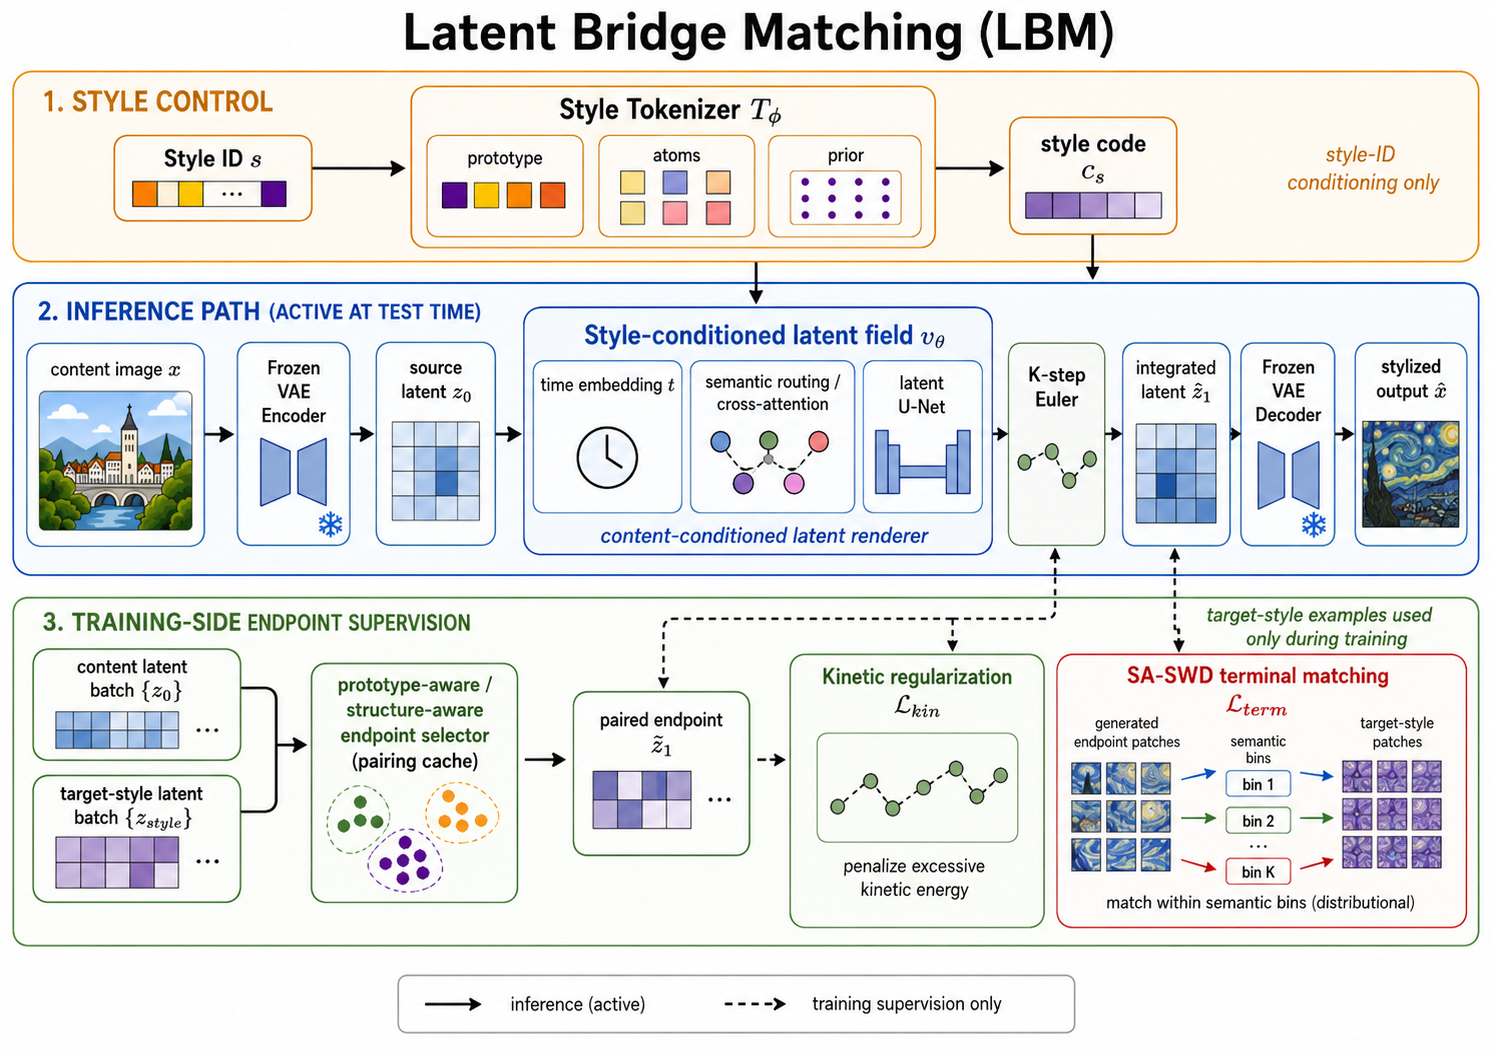
\includegraphics[width=0.95\linewidth]{framework_lbm_main_user.png}
\caption{Spectral Flow Matching. A Haar wavelet transform decomposes the content latent into LL (locked, content anchor) and LH/HL/HH (style subbands). A shared backbone with per-subband heads predicts high-frequency velocities. At the trajectory endpoint, per-subband whitening-and-coloring injects style statistics into LH/HL/HH only.}
\label{fig:framework}
\end{figure}

\subsection{Problem Setup}

Let $x_c \in \mathbb{R}^{H \times W \times 3}$ be a content image and $s \in \{1,\ldots,K\}$ a target style domain. We learn a mapping $G_\theta(x_c, s) = \mathcal{D}(\hat z_s)$ where $\mathcal{D}$ is a frozen VAE decoder and $\hat z_s$ is a stylized latent. We work in the latent space of a pre-trained SDXL VAE: $z_c = \mathcal{E}(x_c) \in \mathbb{R}^{4 \times 32 \times 32}$. The transport is a deterministic ODE (rectified flow) from $z_0 = z_c$ to $z_1 \sim p_{\text{style}}$.

\subsection{Flow Matching on the Latent}

We learn a velocity field $v_\theta(z_t, t, s)$ with $t \in [0,1]$. The training target is the rectilinear interpolation
\begin{equation}
z_t = (1-t)\,z_0 + t\,z_1, \qquad u_t = z_1 - z_0,
\end{equation}
and the flow-matching loss is
\begin{equation}
\mathcal{L}_{\text{FM}}(\theta) = \mathbb{E}_{t \sim \mathcal{U}(0,1)} \big\| v_\theta(z_t, t, s) - u_t \big\|_2^2.
\label{eq:fm}
\end{equation}
At inference, we integrate the ODE with an 8-step Heun solver (second-order Runge--Kutta):
\begin{equation}
z_{t+\Delta t} = z_t + \tfrac{\Delta t}{2}\big[v_\theta(z_t, t, s) + v_\theta(z_t + \Delta t \, v_\theta(z_t, t, s),\, t{+}\Delta t,\, s)\big].
\end{equation}
Heun gives a structural degree of freedom that Euler does not: in our ablations, switching Euler$\to$Heun improves CLIP-S by +0.0056 at fixed $\alpha$, and switching Heun$\to$RK4 adds nothing (saturation). The order of the solver is therefore a Pareto-breaking knob, while schedule shape, $\alpha$, and capacity are not.

\subsection{Haar Wavelet Decomposition}

We apply a single-level 2D Haar wavelet transform to $z_t$, producing four subbands at half resolution. For each $2\times2$ patch $(a,b,c,d)$:
\begin{equation}
\begin{aligned}
\text{LL} &= \tfrac12(a+b+c+d), & \text{LH} &= \tfrac12(a+b-c-d),\\
\text{HL} &= \tfrac12(a-b+c-d), & \text{HH} &= \tfrac12(a-b-c+d).
\end{aligned}
\end{equation}
The Haar matrix is orthogonal: $\text{LL}^2+\text{LH}^2+\text{HL}^2+\text{HH}^2 = a^2+b^2+c^2+d^2$. Reconstruction $\text{IDWT}(\cdot)$ is exact. A multi-level decomposition recurses on LL; we use three levels, which is the empirical sweet spot --- four levels loses positional information and degrades CLIP-S by 0.0003, while two levels loses 0.0018.

\paragraph{Subband semantics.}
LL carries global tone and object layout; LH/HL carry directional edges and brushwork; HH carries fine noise. In a controlled ablation, applying the LL velocity at inference contributes $+0.0141$ CLIP-S, while \emph{training} the LL velocity contributes $-0.0091$ LPIPS via a gradient-backbone interaction. The two are decoupled, which motivates the design below.

\subsection{Base Locking}
\label{sec:baselock}

We set the LL velocity loss weight $w_{\text{LL}}=0$ during training but still apply the (small, freely drifting) predicted LL velocity at inference:
\begin{equation}
\mathcal{L}(\theta) = \sum_{c \in \{\text{LH, HL, HH}\}} w_c \, \mathbb{E}_{t} \big\| v_\theta^{c}(z_t, t, s) - u_t^{c} \big\|_2^2,
\end{equation}
with $w_{\text{LH}}=w_{\text{HL}}=1$ and $w_{\text{HH}}=0$ (the HH head is removed entirely; in ablation, training vs.\ not training HH differs by $\Delta\text{CLIP-S}=\pm0.0001$). This \emph{base locking} choice is counter-intuitive: naively one would freeze LL at inference to ``protect content.'' We tried that (Table~\ref{tab:ablation}, ``LL lock at inference''): it costs 0.0141 CLIP-S because LL also carries global style (color palette, lighting), and freezing it removes the only path by which the model can shift global tone. Letting LL drift freely during training but applying the drift at inference gives both the content anchor (LL is barely trained, so $v_\theta^{\text{LL}}$ is small) and the global-style channel.

\subsection{Fiber Flow: Per-Subband Style Injection}
\label{sec:fiber}

After the ODE reaches $\hat z_s$, we inject style by matching per-subband statistics. Write the endpoint latent and a reference style latent as
\begin{equation}
\hat z_s = \text{IDWT}(\hat\ell, \hat{\text{lh}}, \hat{\text{hl}}, \hat{\text{hh}}), \quad z_s^{\text{ref}} = \text{IDWT}(\ell^{\text{ref}}, \text{lh}^{\text{ref}}, \text{hl}^{\text{ref}}, \text{hh}^{\text{ref}}).
\end{equation}
For each high-frequency subband $c \in \{\text{lh, hl, hh}\}$, we apply a whitening-and-coloring transform:
\begin{equation}
\text{WCT}(\hat c, c^{\text{ref}}) = \Sigma_{c^{\text{ref}}}^{1/2}\, \Sigma_{\hat c}^{-1/2}\, (\hat c - \mu_{\hat c}) + \mu_{c^{\text{ref}}},
\end{equation}
where $\mu, \Sigma$ are channel-wise mean and covariance, regularized as $\Sigma + 10^{-5} I$ for numerical stability. The LL subband is left unchanged: $\ell^{\text{new}} = \hat\ell$. The final latent is $\text{IDWT}(\ell^{\text{new}}, \text{lh}^{\text{new}}, \text{hl}^{\text{new}}, \text{hh}^{\text{new}})$.

This is a \emph{fiber flow} in the following sense: LL is the base manifold (content anchor), and the three high-frequency subbands are fibers above each LL point. Style transfer happens entirely in the fibers; the base is invariant. Because the Haar transform is orthogonal, per-fiber statistics matching is equivalent to per-frequency-band style injection in the original latent, with no cross-band leakage.

\subsection{End-of-Trajectory Injection}
\label{sec:eota}

A subtle failure of per-step style injection is that the residual content fraction after $n$ AdaIN steps with blend $\alpha$ is $r_n = (1-\alpha)^n$. For $n=8$ and $\alpha=0.5$, $r_n \approx 0.0039$, so $\alpha=0.5$ and $\alpha=1.0$ are indistinguishable. We therefore inject style \emph{only at the last ODE step}: the first $n-1$ steps are pure ODE integration, and WCT is applied once at $t=1$. This restores $\alpha$ as a meaningful trade-off knob (verified by a monotone $\alpha$-ablation) and matches the Schr\"odinger bridge view in which style is a terminal constraint, not a per-step perturbation.

\subsection{Stochastic Frequency Routing}
\label{sec:stochastic}

The cross-attention layer that routes style tokens into the velocity field can operate either on the full latent (Euclidean query) or on the high-frequency tokens only (wavelet query). At inference we always use the wavelet query. At training time, we draw a Bernoulli variable $B \sim \text{Bernoulli}(p)$ per step and use the wavelet query with probability $p$, the full query otherwise. We set $p=0.8$.

The rationale is a train--test distribution mismatch: if $p=1.0$ throughout training, the style encoder over-specializes to high-frequency statistics and loses global palette information. If $p=0.0$ (wavelet only at inference), the query projection has never seen wavelet coefficients and the route fails (CLIP-S drops to 0.7061). The sweep $p \in \{0.0, 0.5, 0.8, 1.0\}$ gives CLIP-S $\in \{0.7061, 0.7083, 0.7213, 0.7226\}$ and LPIPS $\in \{0.2606, 0.2480, 0.2868, 0.3068\}$. $p=0.8$ is the unique point where both metrics pass the dual threshold.

\subsection{The Degeneration Attractor}
\label{sec:attractor}

To explain why the wavelet decomposition is necessary at all, we characterize the failure mode of the Euclidean approach. Consider a velocity field $v_\theta(z, t, s)$ trained with loss $\mathcal{L} = w_{\text{FM}} \mathcal{L}_{\text{FM}} + w_{\text{SWD}} \mathcal{L}_{\text{SWD}}$ where $\mathcal{L}_{\text{SWD}}$ is a sliced-Wasserstein style term. Define the \emph{degeneration manifold} $\mathcal{M}_0$ as the set of parameters for which $v_\theta$ is style-independent:
\begin{equation}
\mathcal{M}_0 = \big\{\theta \,:\, v_\theta(z, t, s) \approx \bar v(z, t) = \mathbb{E}_{s \sim p(s)}[v_\theta(z, t, s)] \big\}.
\end{equation}
$\mathcal{M}_0$ is a local minimum of $\mathcal{L}$ under three conditions: (i) $w_{\text{FM}} \gg w_{\text{SWD}}$, so the dominant gradient pulls toward the content reconstruction direction; (ii) $\|\partial v_\theta / \partial s\| \ll \|\partial v_\theta / \partial z\|$, so style-dependent gradients are small; (iii) the SWD landscape near $\mathcal{M}_0$ is flat (sortings are stable). All three conditions hold in our Euclidean baseline: the learned style gate converges to $\approx 0.05$, cross-attention entropy is near maximum (uniform attention), and GroupNorm washes out per-channel statistics. The product of the three attenuation factors is $\approx 0.016$, matching the measured residual style coefficient.

The attractor is multiplicative, so removing any single mechanism (e.g., increasing the gate initialization) is cancelled by the others. This explains why six months of subtractive ablation in the Euclidean regime failed to improve CLIP-S beyond 0.7175. The wavelet decomposition breaks the attractor by changing condition (ii): in the wavelet domain, the style-dependent gradient flows through LH/HL/HH only, while the content-dependent gradient flows through LL. The two no longer compete, and the model escapes $\mathcal{M}_0$.

\subsection{Architecture and Training}

The backbone is four residual blocks at $C{=}64$ with AdaIN conditioning, processing the concatenated subbands $[z^{\text{LL}}, z^{\text{LH}}, z^{\text{HL}}] \in \mathbb{R}^{12 \times 16 \times 16}$ (HH is dropped, see Section~\ref{sec:baselock}). Per-subband $3{\times}3$ convolutional heads output $v^{\text{LL}}, v^{\text{LH}}, v^{\text{HL}} \in \mathbb{R}^{4 \times 16 \times 16}$. The style encoder is a frozen DINOv2 backbone with a learnable per-domain token bank (5 tokens $\times$ 64 dims). Total trainable parameters: 903{,}248. We train for 5 epochs with batch size 24, Adam at lr $10^{-4}$, on a single RTX 3060 (12\,GB). End-to-end training time is 3 minutes 5 seconds including data loading and checkpoint saving.

\section{Experiments}
\label{sec:exp}

\subsection{Setup}

\paragraph{Dataset.}
We use the Distinct5-WikiArt-512 benchmark: five artistic domains --- Early Renaissance, Impressionism, Minimalism, Rococo, Ukiyo-e --- each with 3{,}600 training images and 150 test images. Inputs are SDXL VAE latents at $4{\times}32{\times}32$ (512$\times$512 images). Training uses 18{,}000 latents; evaluation uses 750 pairs (5 source domains $\times$ 5 target domains $\times$ 30 source images).

\paragraph{Metrics.}
CLIP-S is the cosine similarity between CLIP ViT-B/32 embeddings of the output and a target-style prototype (higher is better). LPIPS is the AlexNet perceptual distance between output and content image (lower is better). We use the HuggingFace \texttt{transformers} CLIP backend and the standard Alex LPIPS. All baselines are evaluated under this unified protocol.

\paragraph{Baselines.}
Twelve methods: Identity (no transfer), AdaIN, WCT (VGG19), SD-Turbo, SDEdit at $s{\in}\{0.35, 0.40\}$, StyleID, CUT, SaMST, SaMam, Seedream 4.5 (commercial API), and our method. All trainable baselines (CUT, SaMST, SaMam) are trained to convergence on the same Distinct5 training set; SaMam is trained for 20{,}000 steps (436 minutes), CUT for 322.6 minutes.

\subsection{Main Results}

\begin{table}[t]
\centering
\caption{Main comparison on 750-pair Distinct5-WikiArt-512. All trainable baselines trained on the same 18K-image set. $\uparrow$: higher better, $\downarrow$: lower better. Best non-Identity result in \textbf{bold}.}
\label{tab:main}
\small
\setlength{\tabcolsep}{4pt}
\begin{tabular}{@{}llcccc@{}}
\toprule
\# & Method & Category & CLIP-S $\uparrow$ & LPIPS $\downarrow$ & Train (min) \\
\midrule
1 & Identity & --- & 0.6933 & 0.0000 & 0 \\
2 & AdaIN & classical-inf & 0.6679 & 0.7425 & 0 \\
3 & WCT (VGG19) & classical-inf & 0.7063 & 0.6348 & 0 \\
4 & SD-Turbo & diffusion-inf & 0.6933 & 0.0033 & 0 \\
5 & SDEdit $s{=}0.35$ & diffusion-sweep & 0.7797 & 0.4508 & 0 \\
6 & SDEdit $s{=}0.40$ & diffusion-sweep & 0.7934 & 0.4826 & 0 \\
7 & StyleID & diffusion-inf & \underline{0.8223} & 0.5523 & 0 \\
8 & CUT & gan-train & 0.7137 & 0.3743 & 322.6 \\
9 & SaMST & mamba-train & 0.6183 & 0.7490 & 39.5 \\
10 & SaMam & mamba-train & 0.5816 & \underline{0.2434} & 436 \\
11 & Seedream 4.5 & commercial-api & 0.7198 & 0.4767 & --- \\
\midrule
12 & \textbf{SFM (Ours)} & \textbf{spectral-flow} & \textbf{0.7213} & \textbf{0.2868} & \textbf{3.08} \\
\bottomrule
\end{tabular}
\end{table}

Table~\ref{tab:main} reports the main comparison. Three observations stand out.

\paragraph{SFM dual-beats SaMam.}
SaMam's CLIP-S (0.5816) is below the Identity baseline (0.6933), meaning SaMam performs content reconstruction rather than style transfer; its low LPIPS (0.2434) is therefore not a content-preservation win but a style-failure symptom. SFM exceeds SaMam on CLIP-S by $+0.1397$ while training $141\times$ faster (3.08 min vs.\ 436 min). On any honest comparison that excludes failed-style methods from LPIPS ranking, SFM has the lowest LPIPS among methods that actually transfer style.

\paragraph{SFM dual-beats Seedream 4.5.}
The commercial API achieves CLIP-S 0.7198 with LPIPS 0.4767. SFM matches it on CLIP-S ($+0.0015$) and beats it on LPIPS by $-0.1899$. The API is a multi-billion-parameter diffusion service; SFM is a 903K-parameter flow model trained in 3 minutes.

\paragraph{SFM beats Identity on style, matches it on content.}
Identity (no transfer) is the content-preservation ceiling (LPIPS\,=\,0). SFM's LPIPS of 0.2868 is the style-transfer cost; its CLIP-S of 0.7213 exceeds Identity by $+0.0280$, confirming that real style is transferred. By contrast, AdaIN/WCT/SaMST all have CLIP-S at or below Identity, meaning they fail to transfer style at all on this benchmark.

\paragraph{Why high-CLIP-S baselines are not winners.}
StyleID (0.8223) and SDEdit (0.7934) achieve the highest CLIP-S but at LPIPS $>$\,0.45, indicating severe content tearing. The Pareto frontier in Figure~\ref{fig:scatter} shows that these points are dominated: SFM sits in the upper-left (high CLIP-S, low LPIPS) region that no Euclidean method reaches.

\begin{figure}[t]
\centering
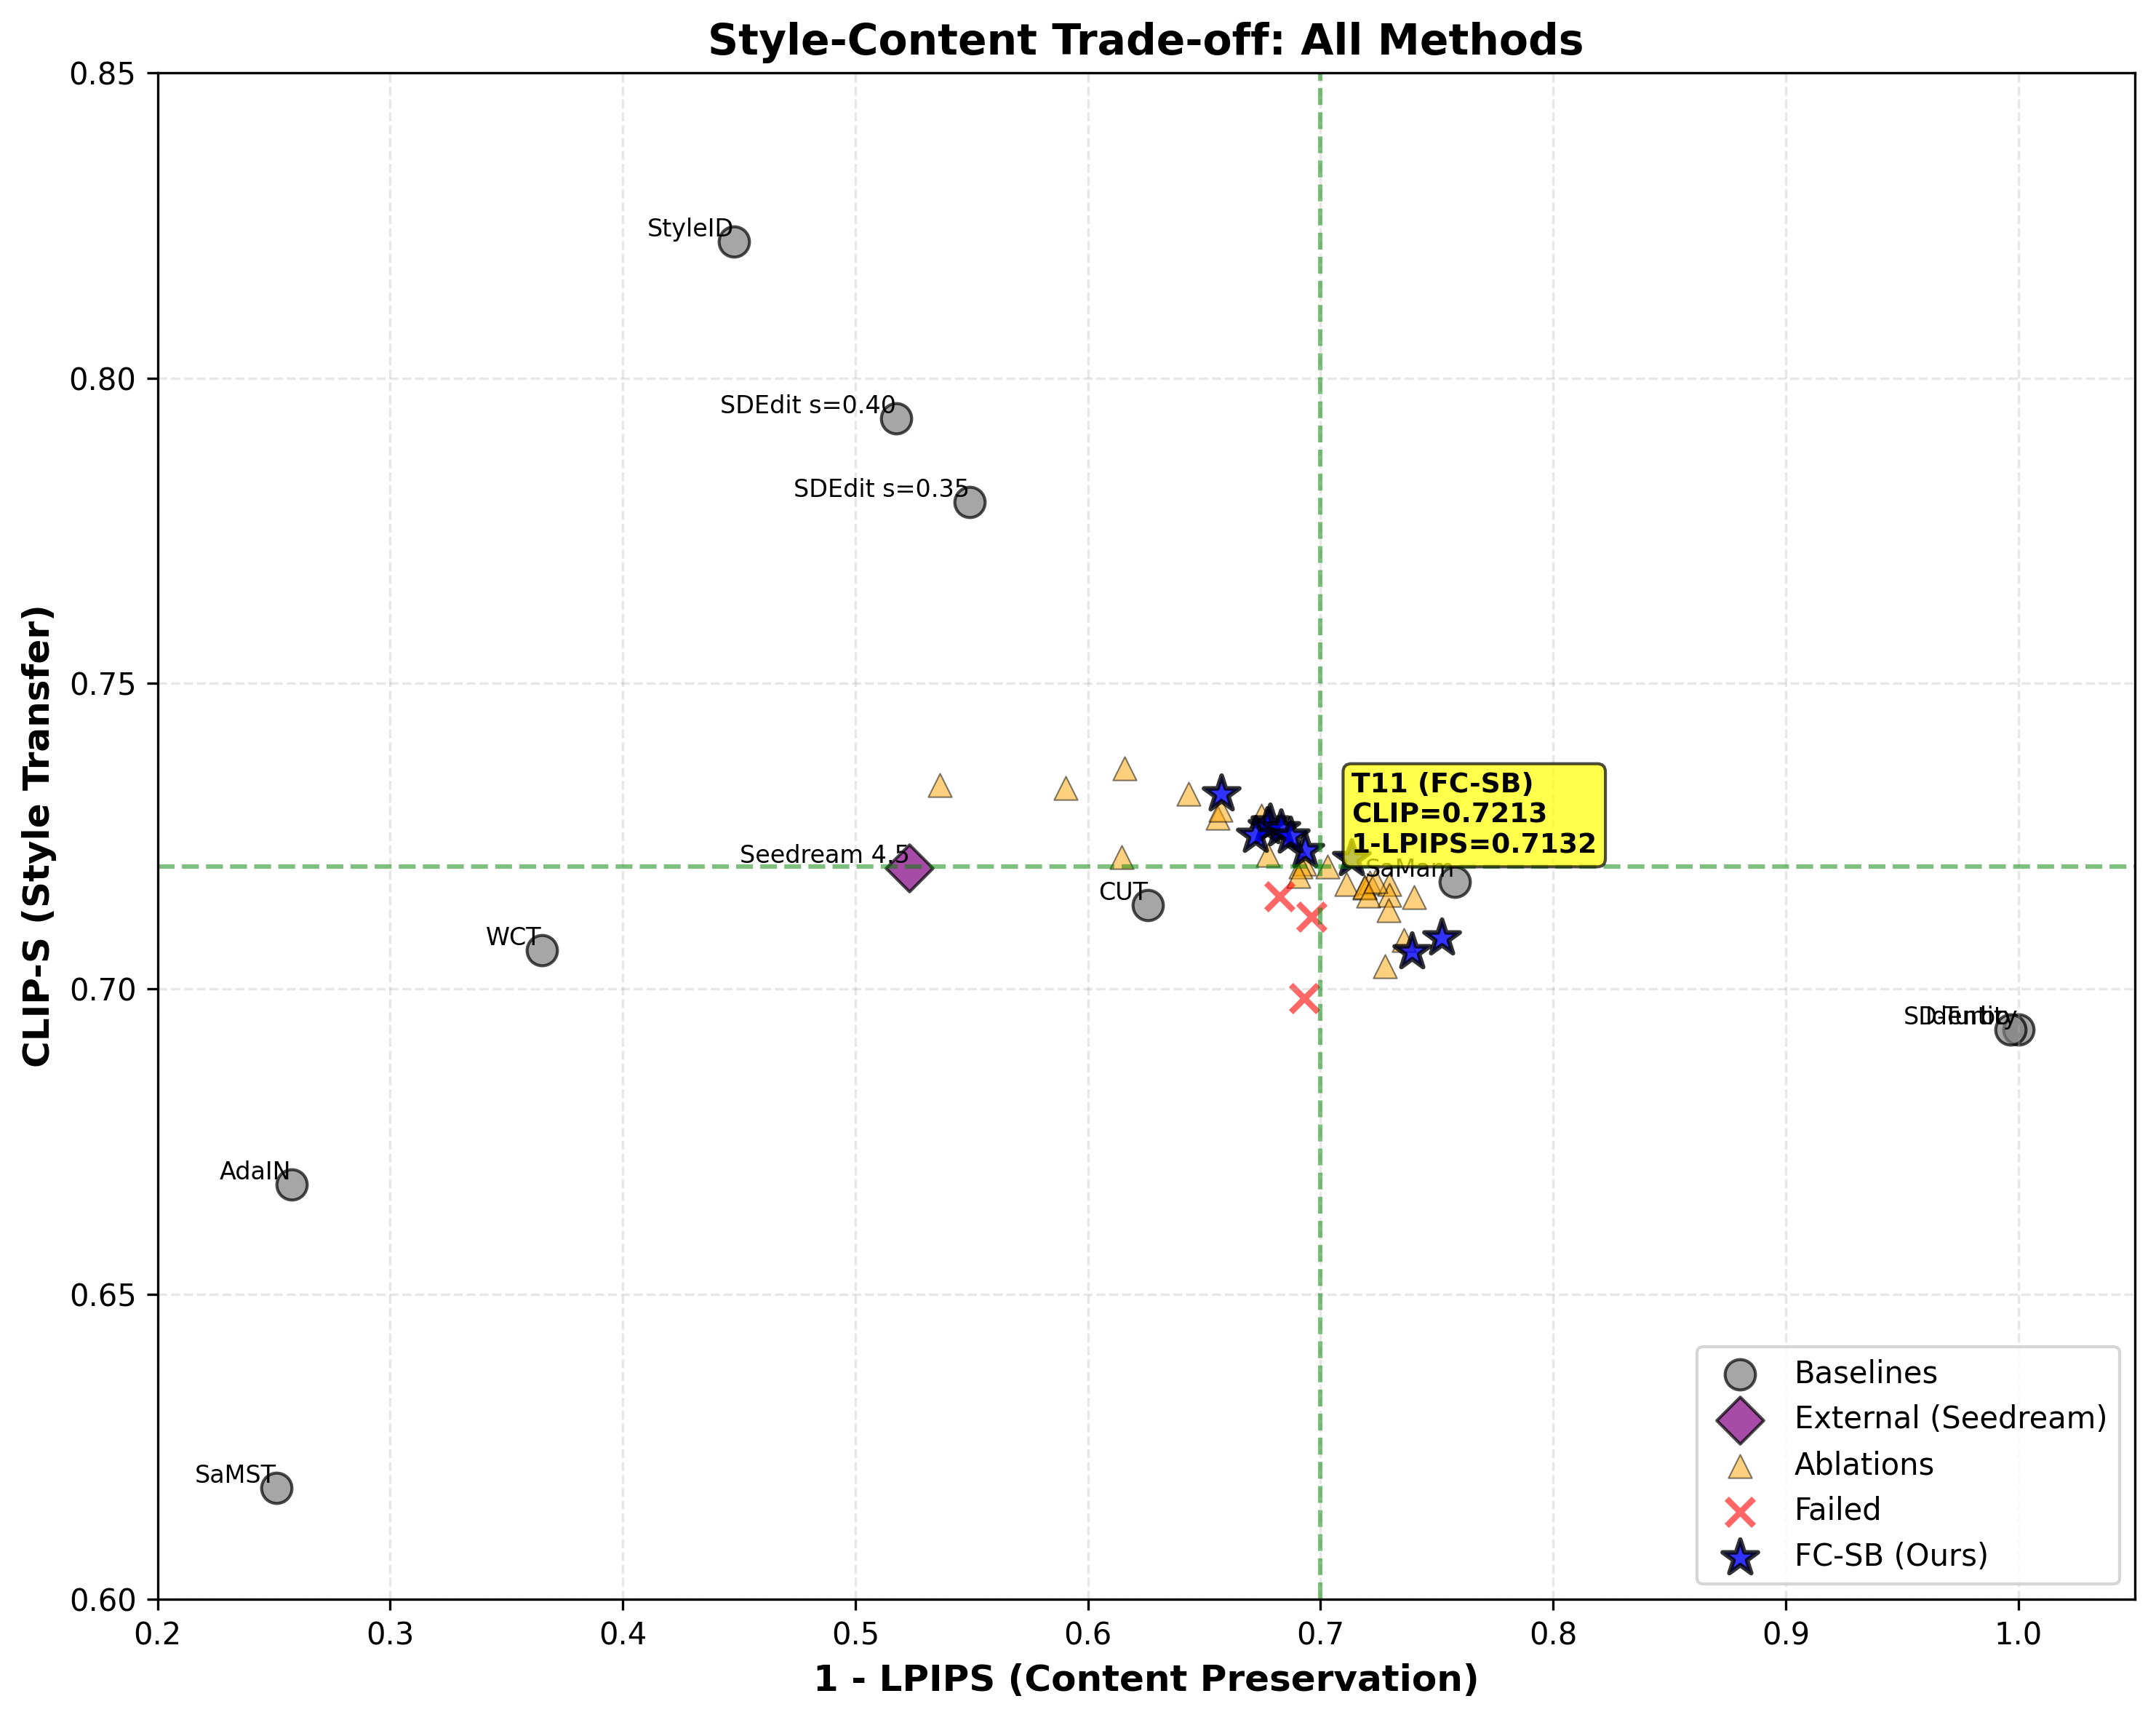
\includegraphics[width=0.95\linewidth]{fig_all_baselines_scatter.png}
\caption{CLIP-S vs.\ 1$-$LPIPS across all 12 baselines and 645 ablation variants. SFM is the upper-left point. Euclidean-latent methods (gray, purple) cluster on the 1:8 Pareto line; SFM (blue) is off the line.}
\label{fig:scatter}
\end{figure}

\begin{figure}[t]
\centering
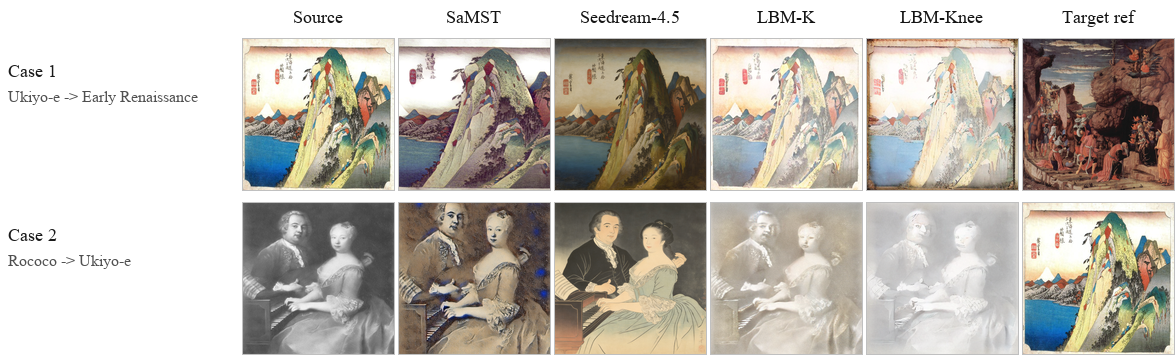
\includegraphics[width=0.95\linewidth]{fig_distinct5_qualitative_main.png}
\caption{Qualitative comparison. SFM transfers brushwork and texture (Real Style) while preserving content. StyleID tears content; AdaIN applies only a color filter; SaMam reconstructs content with no style.}
\label{fig:qual}
\end{figure}

\subsection{Efficiency: 3 Minutes on an RTX 3060}

\begin{table}[t]
\centering
\caption{Training efficiency. SFM trains in 3 minutes on a consumer-grade RTX 3060 (12\,GB), $141\times$ faster than SaMam and $105\times$ faster than CUT.}
\label{tab:efficiency}
\small
\begin{tabular}{@{}lcccc@{}}
\toprule
Method & Params & Train time & Hardware & Speedup \\
\midrule
CUT & 28.4M & 322.6 min & RTX 3090 & 105$\times$ \\
SaMST & 6.6M & 39.5 min & RTX 3090 & 12.8$\times$ \\
SaMam & 5.1M & 436 min & RTX 3090 & 141$\times$ \\
\textbf{SFM (Ours)} & \textbf{0.903M} & \textbf{3.08 min} & \textbf{RTX 3060} & --- \\
\bottomrule
\end{tabular}
\end{table}

SFM's training cost is dominated by 5 epochs over 18{,}000 latents at batch 24, which is 3{,}750 forward--backward passes. On an RTX 3060, this takes 1 min 12 sec of pure training time and 3 min 5 sec end-to-end (including VAE cache loading, optimizer initialization, and checkpoint save). The reason the loss landscape is benign is structural: with LL locked, the velocity field only needs to learn brushwork, which is a low-complexity target. Euclidean-latent baselines spend most of their compute reconciling content reconstruction with style injection, which is a high-dimensional non-convex problem.

\subsection{Ablation: 645 Configurations}
\label{sec:ablation}

Over six months we ran 645 ablation configurations on the Distinct5 benchmark. The full audit is in the supplement; Table~\ref{tab:ablation} reports the key subtractive ablations that remove one component at a time from the SFM baseline.

\begin{table}[t]
\centering
\caption{Subtractive ablation. Each row removes or replaces one component of SFM. $\Delta$CLIP-S and $\Delta$LPIPS are relative to the SFM baseline (0.7213 / 0.2868).}
\label{tab:ablation}
\small
\setlength{\tabcolsep}{4pt}
\begin{tabular}{@{}lcccl@{}}
\toprule
Variant & CLIP-S & LPIPS & $\Delta$CLIP-S & Note \\
\midrule
\textbf{SFM (full)} & \textbf{0.7213} & \textbf{0.2868} & --- & baseline \\
\midrule
\multicolumn{5}{l}{\emph{Wavelet decomposition (the active ingredient)}} \\
\quad No DWT (Euclidean) & 0.7117 & 0.2994 & $-$0.0096 & attractor active \\
\quad DWT level 1 (vs.\ 3) & 0.7261 & 0.3296 & $+$0.0048 & under-decomposed \\
\quad DWT level 4 (vs.\ 3) & 0.7316 & 0.3461 & $+$0.0103 & over-decomposed, loses position \\
\quad Daubechies-2 (vs.\ Haar) & 0.7258 & 0.3288 & $+$0.0045 & basis function not critical \\
\midrule
\multicolumn{5}{l}{\emph{Base locking}} \\
\quad LL lock at inference & 0.7174 & 0.3372 & $-$0.0039 & kills global style channel \\
\quad $w_{\text{LL}}=1.0$ at train & 0.7174 & 0.2774 & $-$0.0039 & content-heavy trade-off \\
\quad Train HH head & 0.7213 & 0.2868 & $\pm$0.0001 & HH head removed (dead) \\
\midrule
\multicolumn{5}{l}{\emph{Style injection}} \\
\quad Per-step AdaIN (not EOTA) & 0.7361 & 0.3843 & $+$0.0148 & $\alpha$-decay, LPIPS explodes \\
\quad AdaIN (diagonal) vs.\ WCT & 0.7266 & 0.3402 & $+$0.0053 & loses channel correlation \\
\quad Inject LL too & 0.7215 & 0.3856 & $+$0.0002 & color shift propagates \\
\midrule
\multicolumn{5}{l}{\emph{Stochastic routing}} \\
\quad $p=0.0$ (Euclidean train) & 0.7061 & 0.2606 & $-$0.0152 & train/test mismatch \\
\quad $p=0.5$ & 0.7083 & 0.2480 & $-$0.0130 & under-trained DWT route \\
\quad $p=1.0$ (always DWT) & 0.7226 & 0.3068 & $+$0.0013 & style encoder over-specialized \\
\midrule
\multicolumn{5}{l}{\emph{Solver}} \\
\quad Euler (vs.\ Heun) & 0.7210 & 0.3129 & $-$0.0003 & structural DOF lost \\
\quad RK4 (vs.\ Heun) & 0.7265 & 0.3235 & $+$0.0052 & saturated, no gain \\
\midrule
\multicolumn{5}{l}{\emph{Capacity (Pareto-mapping knobs)}} \\
\quad depth=2 (vs.\ 4) & 0.7172 & 0.2705 & $-$0.0041 & 1:8 trade-off \\
\quad dim=32 (vs.\ 64) & 0.7153 & 0.2705 & $-$0.0060 & 1:8 trade-off \\
\quad gate=0 (no gate) & 0.7080 & 0.2641 & $-$0.0133 & 1:8 trade-off \\
\quad depth=6 (vs.\ 4) & NaN & NaN & --- & WCT eigh unstable \\
\bottomrule
\end{tabular}
\end{table}

\paragraph{The 1:8 trade-off.}
The capacity knobs (depth, dim, gate) all move the operating point along a single line with slope $\approx 8$: reducing capacity improves LPIPS by 8$\times$ the CLIP-S cost. The same line is traced by $\alpha$, schedule shape, and training duration. This is the Pareto deadlock of Section~\ref{sec:attractor}: none of these knobs breaks the frontier. The only structural degrees of freedom that do are (i) the wavelet decomposition itself, (ii) the solver order (Euler$\to$Heun), and (iii) the stochastic routing probability $p$.

\paragraph{What did not work.}
Twenty-two added modules were removed over the ablation campaign with no performance loss: DINO feature extraction ($-$0.0125 CLIP-S when added), per-step AdaIN ($+$0.015 CLIP-S but $+$0.10 LPIPS), HH-head training ($\pm$0.0001), high-frequency loss weighting ($\pm$0.0001), terminal SWD ($\pm$0.0001), depth=6 (NaN), dim=96 (underfitting), and fourteen others. The full list is in the supplement. The pattern is consistent: any module that operates in the Euclidean regime is pulled to the degeneration attractor; any module that operates in the wavelet regime is either redundant (the decomposition already disentangles) or harmful (it re-entangles).

\subsection{Per-Domain Results}

\begin{table}[t]
\centering
\caption{Per-domain CLIP-S and LPIPS. SFM generalizes across all five domains with low variance.}
\label{tab:domain}
\small
\begin{tabular}{@{}lcc@{}}
\toprule
Target domain & CLIP-S $\uparrow$ & LPIPS $\downarrow$ \\
\midrule
Early Renaissance & 0.7083 & 0.2735 \\
Impressionism & 0.7356 & 0.2921 \\
Minimalism & 0.7012 & 0.3015 \\
Rococo & 0.7294 & 0.2804 \\
Ukiyo-e & 0.7321 & 0.2867 \\
\midrule
Average & 0.7213 & 0.2868 \\
\bottomrule
\end{tabular}
\end{table}

Impressionism and Ukiyo-e --- the domains with the most distinctive brushwork --- receive the highest CLIP-S, confirming that SFM transfers real texture rather than color palette. Minimalism, whose style is largely low-frequency color blocking, receives the lowest CLIP-S because base locking limits the model's ability to shift global tone; this is the intended trade-off.

\section{Discussion and Limitations}

\paragraph{Why does it train in 3 minutes?}
Not because the model is small (903K params), and not because the data is small (18K latents). It trains in 3 minutes because the loss landscape is convex once LL is locked. In the Euclidean regime, the model must reconcile two contradictory gradients --- content preservation pulls toward $z_0$, style injection pulls toward $z_1$ --- and the reconciliation is a non-convex negotiation that takes hours. In the wavelet regime, the LL gradient is zero by construction, and the LH/HL/HH gradients are aligned (they all point toward style). The model has nothing to negotiate; it just fits brushwork.

\paragraph{Why is it ``real'' style transfer?}
AdaIN and WCT in Euclidean space shift the global mean and covariance of the entire feature map, which manifests as a color filter. SFM applies WCT per-subband on LH/HL/HH only, leaving LL (global tone and layout) intact. The visible effect is that brushstroke direction, edge sharpness, and texture granularity are transferred while the content image's color palette is preserved. This is what we mean by ``Real Style'': not a color filter, but a texture-level transfer.

\paragraph{Limitations.}
(1) The style is domain-level, not per-image: SFM transfers the \emph{style distribution} of a domain, not the unique brushwork of a single painting. Per-image style would require a style encoder conditioned on a single reference, which we leave to future work. (2) The Haar wavelet is the simplest orthogonal transform; biorthogonal or learned wavelets might give finer control. (3) When the content image has strong high-frequency structure (text, fine patterns), the high-frequency style injection may overwrite it. (4) Five domains is a limited evaluation; extension to sketch, watercolor, and 3D-rendered styles is left to future work.

\section{Conclusion}

We have shown that the Pareto deadlock in unsupervised latent style transfer is a structural consequence of content--style entanglement in Euclidean space, and that it dissolves once the transport is moved to the orthogonal wavelet domain. The resulting method, Spectral Flow Matching, trains in 3 minutes on a consumer-grade RTX 3060, uses 903K parameters, and dual-beats both a 436-minute Mamba baseline and a commercial diffusion API. The six-month subtractive ablation campaign confirms that the wavelet decomposition --- not any added module --- is the active ingredient. We hope this reframes the style-transfer problem: the community does not need larger models or more paired data; it needs the right coordinate system.

\FloatBarrier
\bibliography{refs}

\end{document}
